\documentclass[12pt]{article}
\usepackage[utf8]{inputenc}
\usepackage{cite}
\usepackage[utf8]{inputenc}
\usepackage{graphicx}
\usepackage{amsmath}
\usepackage[margin=0.5in]{geometry}
\pagenumbering{gobble}
%\usepackage{geometry}
\usepackage{pdfpages}
\usepackage{xcolor}
\usepackage{todonotes}
\usepackage{amsmath,amsfonts,amssymb,amsthm,epsfig,epstopdf,titling,url,array}
\setcounter{secnumdepth}{4}
%\usepackage{enumerate}% http://ctan.org/pkg/enumerate
\title{Computational Model of Peri-Personal Space}
\author{Joan Reyero}
%\date{\today}


\bibliographystyle{apalike}
\bibliography{bib}


\begin{document}

\maketitle

\section{Setting up the unisensory neurons}

The unisensory neurons were set up according to the equations given in section 3.1 in the assignment sheet, as  previously presented by \cite{Serino2015} in his supplementary information.

All the parameters used are the ones given in the assignment sheet except for $I_0^s$, the stimuli amplitude, where
\begin{itemize}
    \item $I_0^t = 49.125$ and
    \item $I_0^a = 67.5$
\end{itemize}
for tactile and auditory neurons respectively. 
\begin{figure}[h!]
	\centering
	\hspace*{-0.6in}
	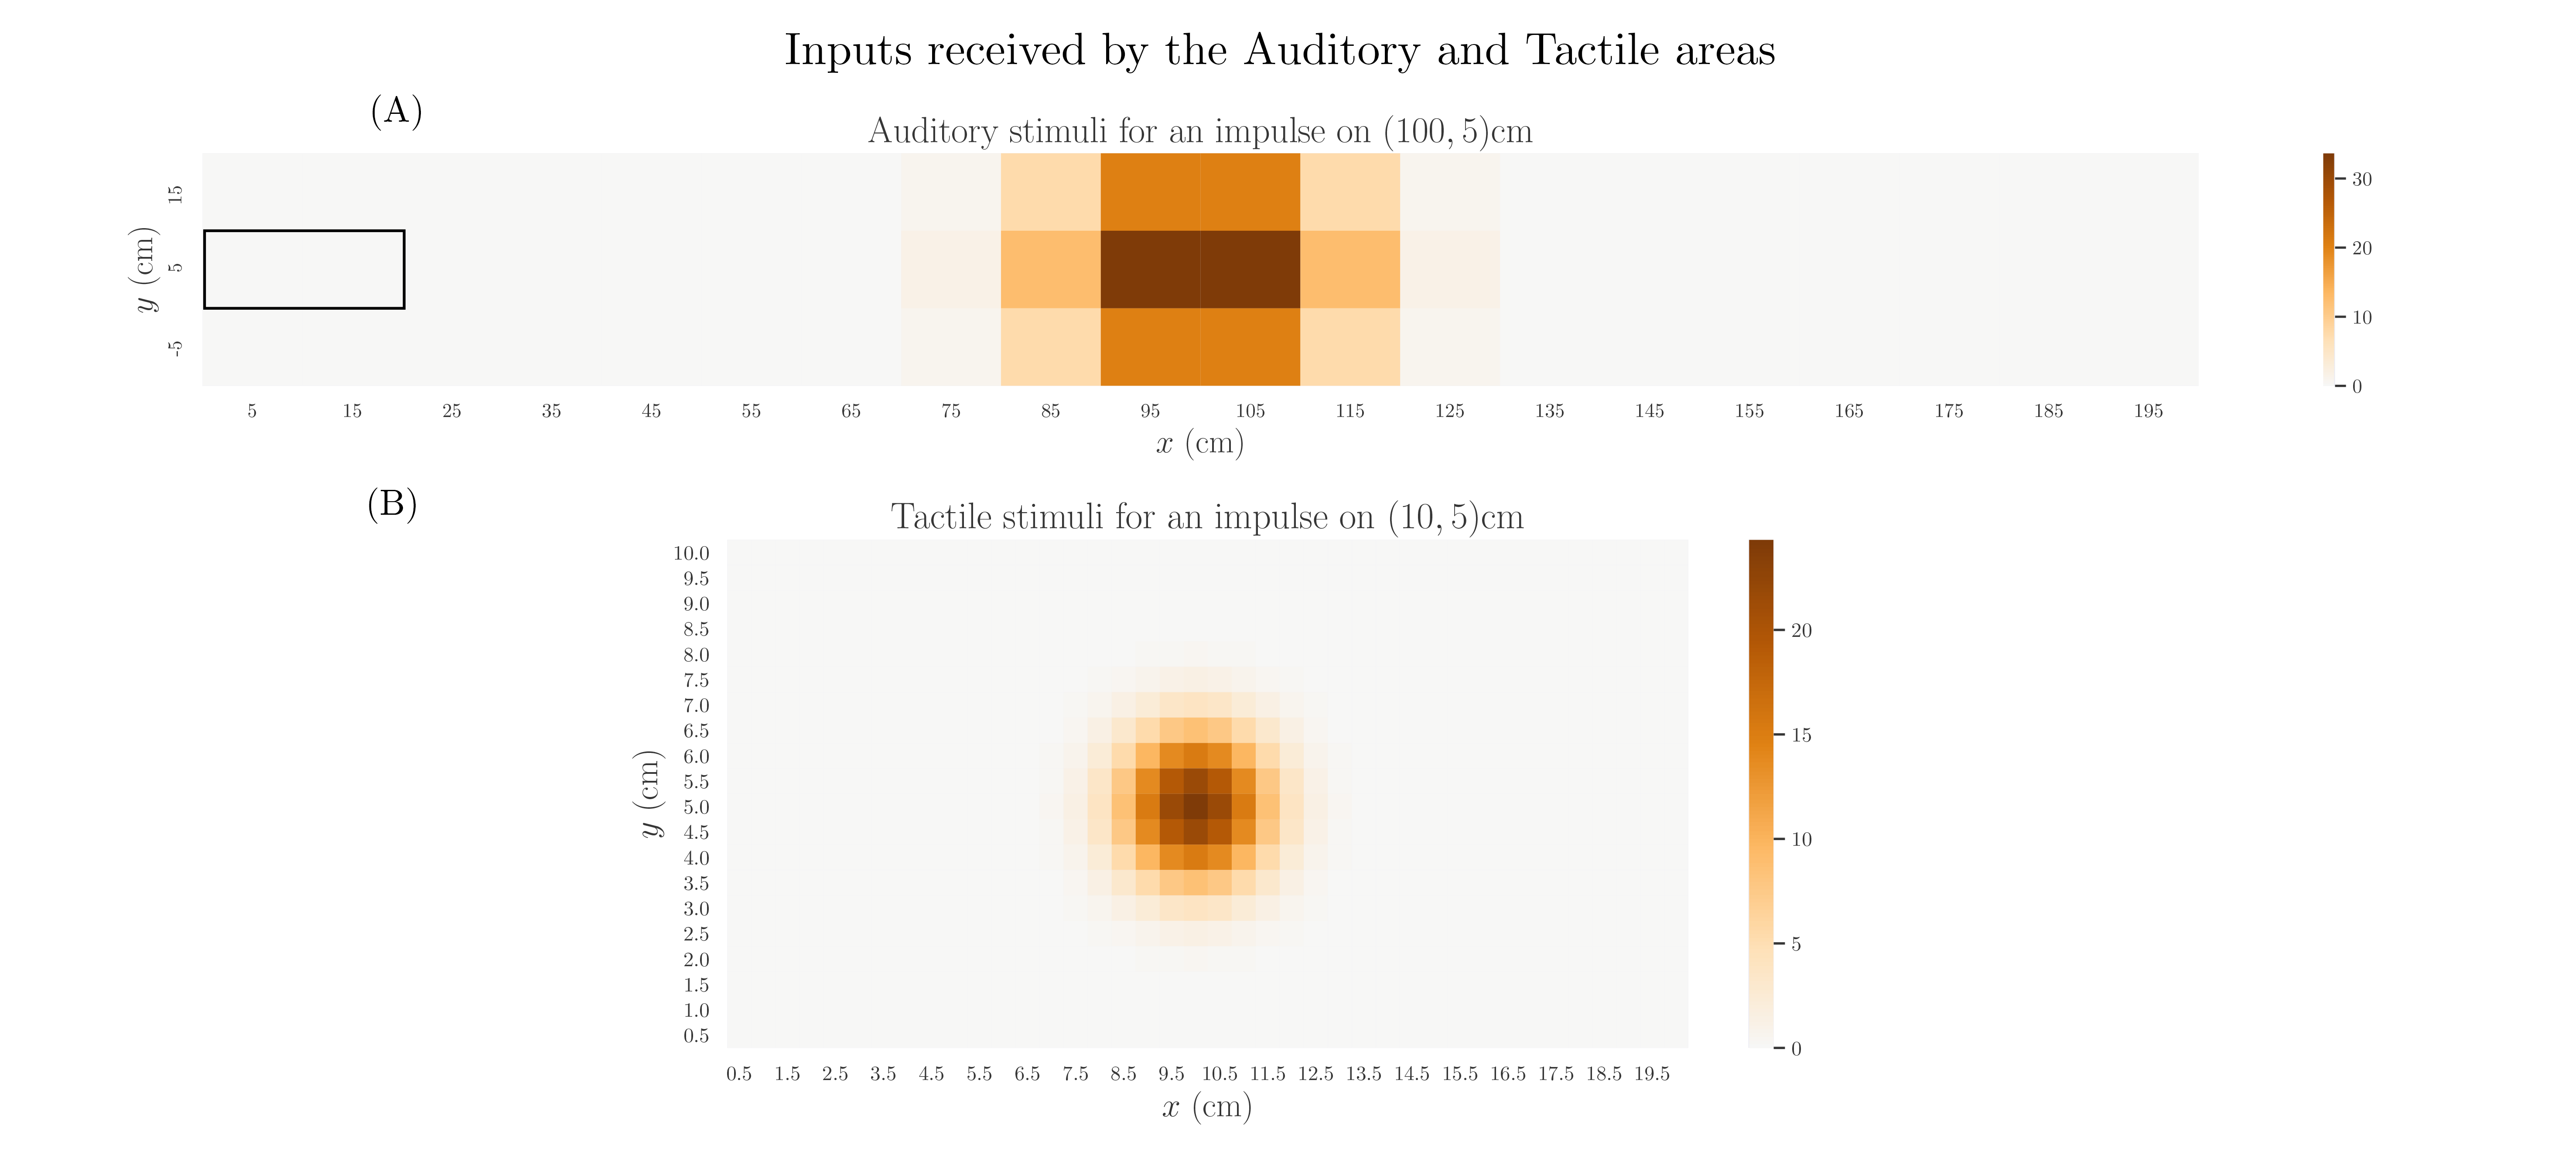
\includegraphics[width=1.2\linewidth]{fig/3-1.png}
	\caption{Inputs received by unisensory neurons. (A) Inputs received by auditory-area neurons for a stimulus placed on $(100,5)$cm. (B) Inputs received by tactile-area neurons for a stimulus placed on $(10,5)$cm, the centre of the tactile area.}
	\label{fig:3.1}
\end{figure}

Figure \ref{fig:3.1} shows the unisensory inputs. Subplots \textit{(A)} and \textit{(B)} show the stimulus on the auditory and tactile areas respectively. It can be seen that the stimulus is felt more dispersely in auditory areas, with a horizontal range from 70 to 130cm. This is largely due to the high spatial extension of the receptive field of the auditory neurons, $\sigma_\phi^a$, which is set to 10cm. In tactile areas, however, the stimulus is much more concentrated, with only 3cm in diamater and a receptive field spacial extension of $\sigma_\phi^a = 1$cm.

\section{Setting connections between neurons}

\subsection{Lateral connectivity in unisensory area}

Neurons in the same area are all connected to each other using lateral connections. The connections follow a mexican-hat type of connectivity: neurons close to each other excite each other, while neurons far from each other inhibit each other.

All the parameters used to model these connectivities are as in the assignment sheet, except for the spatial extension of the tactile inhibitory function, $\sigma_{in}^t$, which was set to instead of 1. This decision was made because, according to \cite{Serino2015}'s supplementary information, in order to have the mexican-hat type of connectivity as a difference of two gaussians, two conditions need to be met: $L_{ex}^s > L_{in}^s$ and $\sigma_{ex}^s < \sigma_{in}^s$; therefore $\sigma_{in}^s$ was set to 4 to match the paper.

\begin{figure}[h!]
	\centering
	\hspace*{-0.6in}
	
\includegraphics[width=1.2\linewidth]{fig/3-2-1.png}
	\caption{Lateral connections for a tactile neuron located at $(10,5)$. The mexican-hat connectivity can be observed, as the neurons close to it are being excited, while the neurons that are further away are being inhibited.}
	\label{fig:3.2.1}
\end{figure}

The results of plotting the response of a neuron located in the central tactile area, in coordinates $(10,15$cm can be seen in figure \ref{fig:3.2.1}. It can be observed that the neuron that is being examined is not exciting iteself, but it is exciting the neurons close to it. Finally, after a threshold of about 3 neurons neurons start being inhibited, with decreasing intensity as we move away from the center.

\subsection{Feedforward and Feedback connectivities}

The feedforward and feedback connectivities were implemented as specified in the assignment sheet.

\begin{figure}[h!]
	\centering
	\hspace*{-0.6in}
	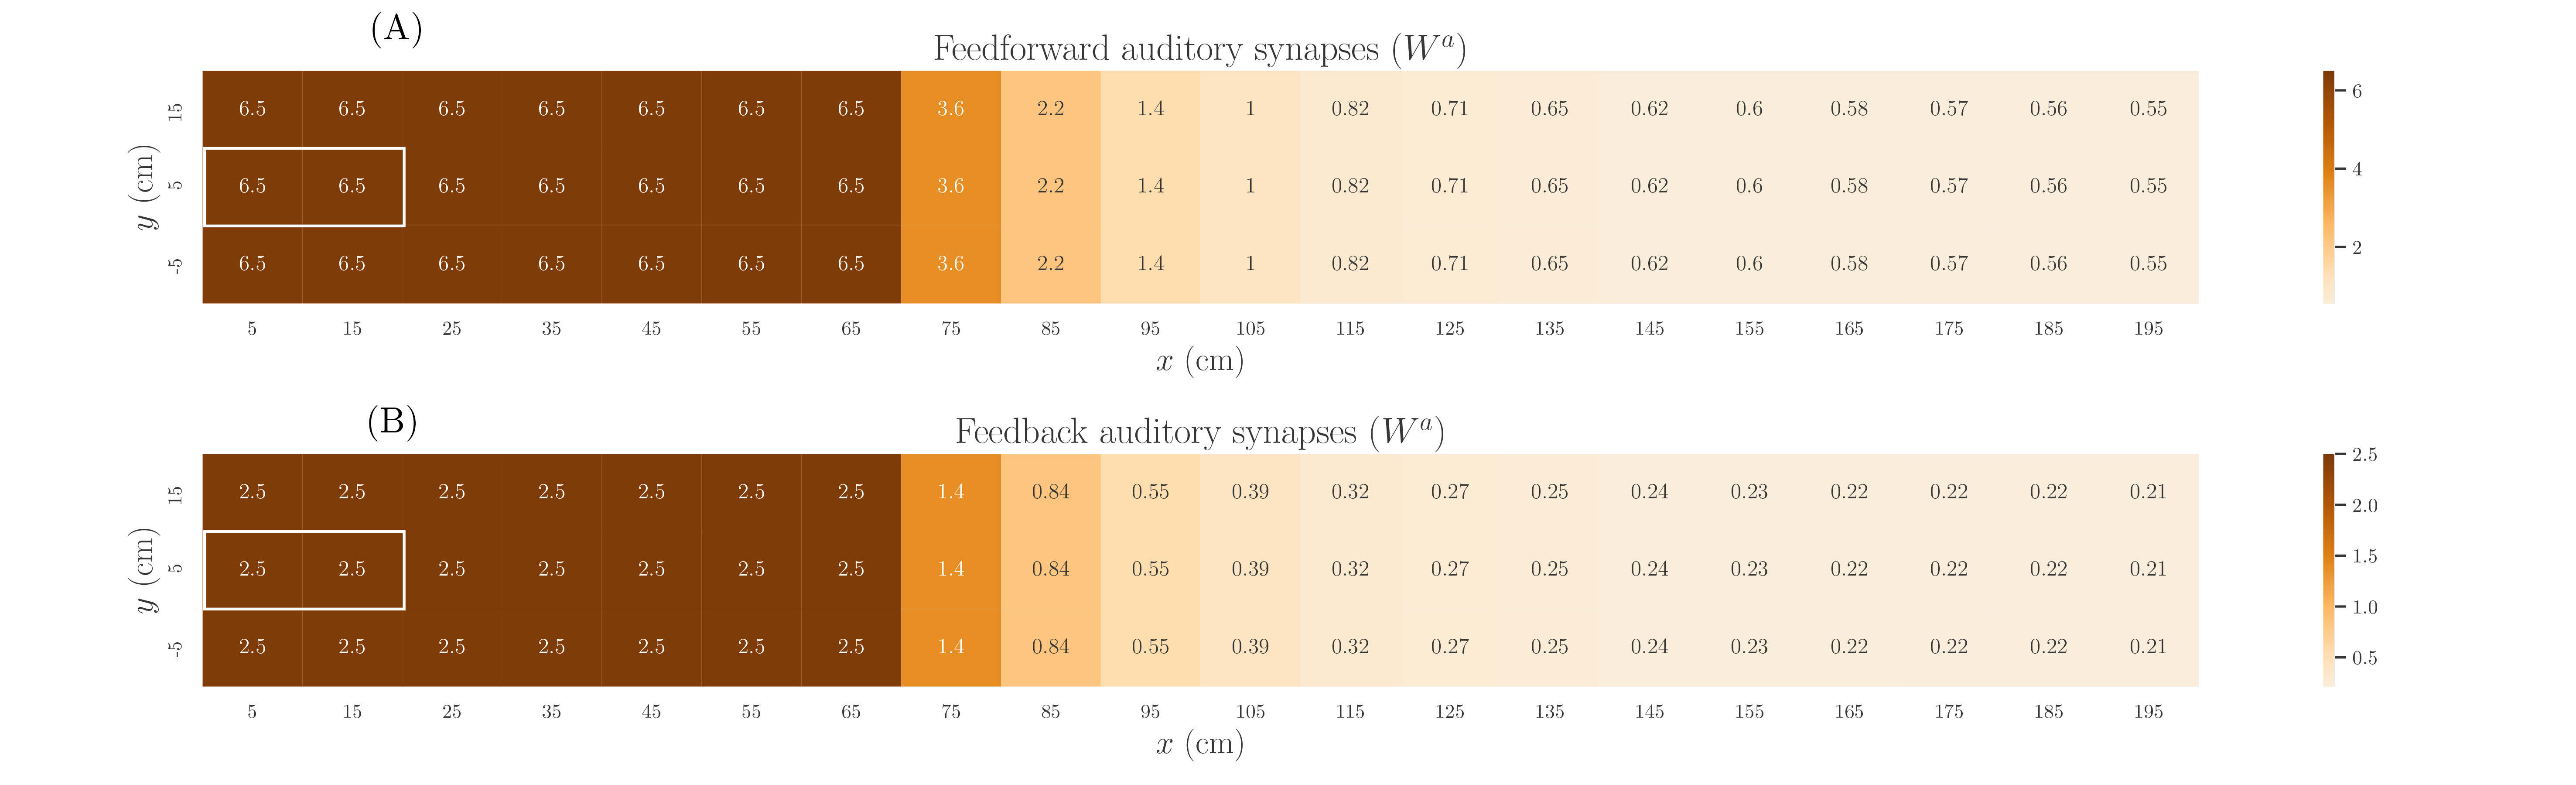
\includegraphics[width=1.2\linewidth]{fig/3-2-2.png}
	\caption{Feedforward \textit{(A)} and Feedback \textit{(B)} connections between the auditory and multisensory areas.}
	\label{fig:3.2.2}
\end{figure}

Figure \ref{fig:3.2.2} shows \textit{(A)} the feedforward connectivities and \textit{(B)} the feedback connectivities between the auditory area and the multisensory area.

\section{Responses of neurons}

\subsection{Responses of unisensory neurons}

The responses of the unisensory neurons were obtained using the differtial equation for the dynamic state of each neuron presented in the assignment sheet. The rate of the neurons was obtained by running the values of the dynamic state through a sigmoidal function.

Figure \ref{fig:3.3.1} shows the response of the auditory area neurons \textit{(A)} for a stimulus placed at $(100, 5)$cm, and the response of the tactile are neurons \textit{(B)} for a stimulus placed at $(10, 5)$cm. Both figures show the rate of the neurons 200ms after the stimulus is presented.

\begin{figure}[h!]
	\centering
	\hspace*{-0.6in}
	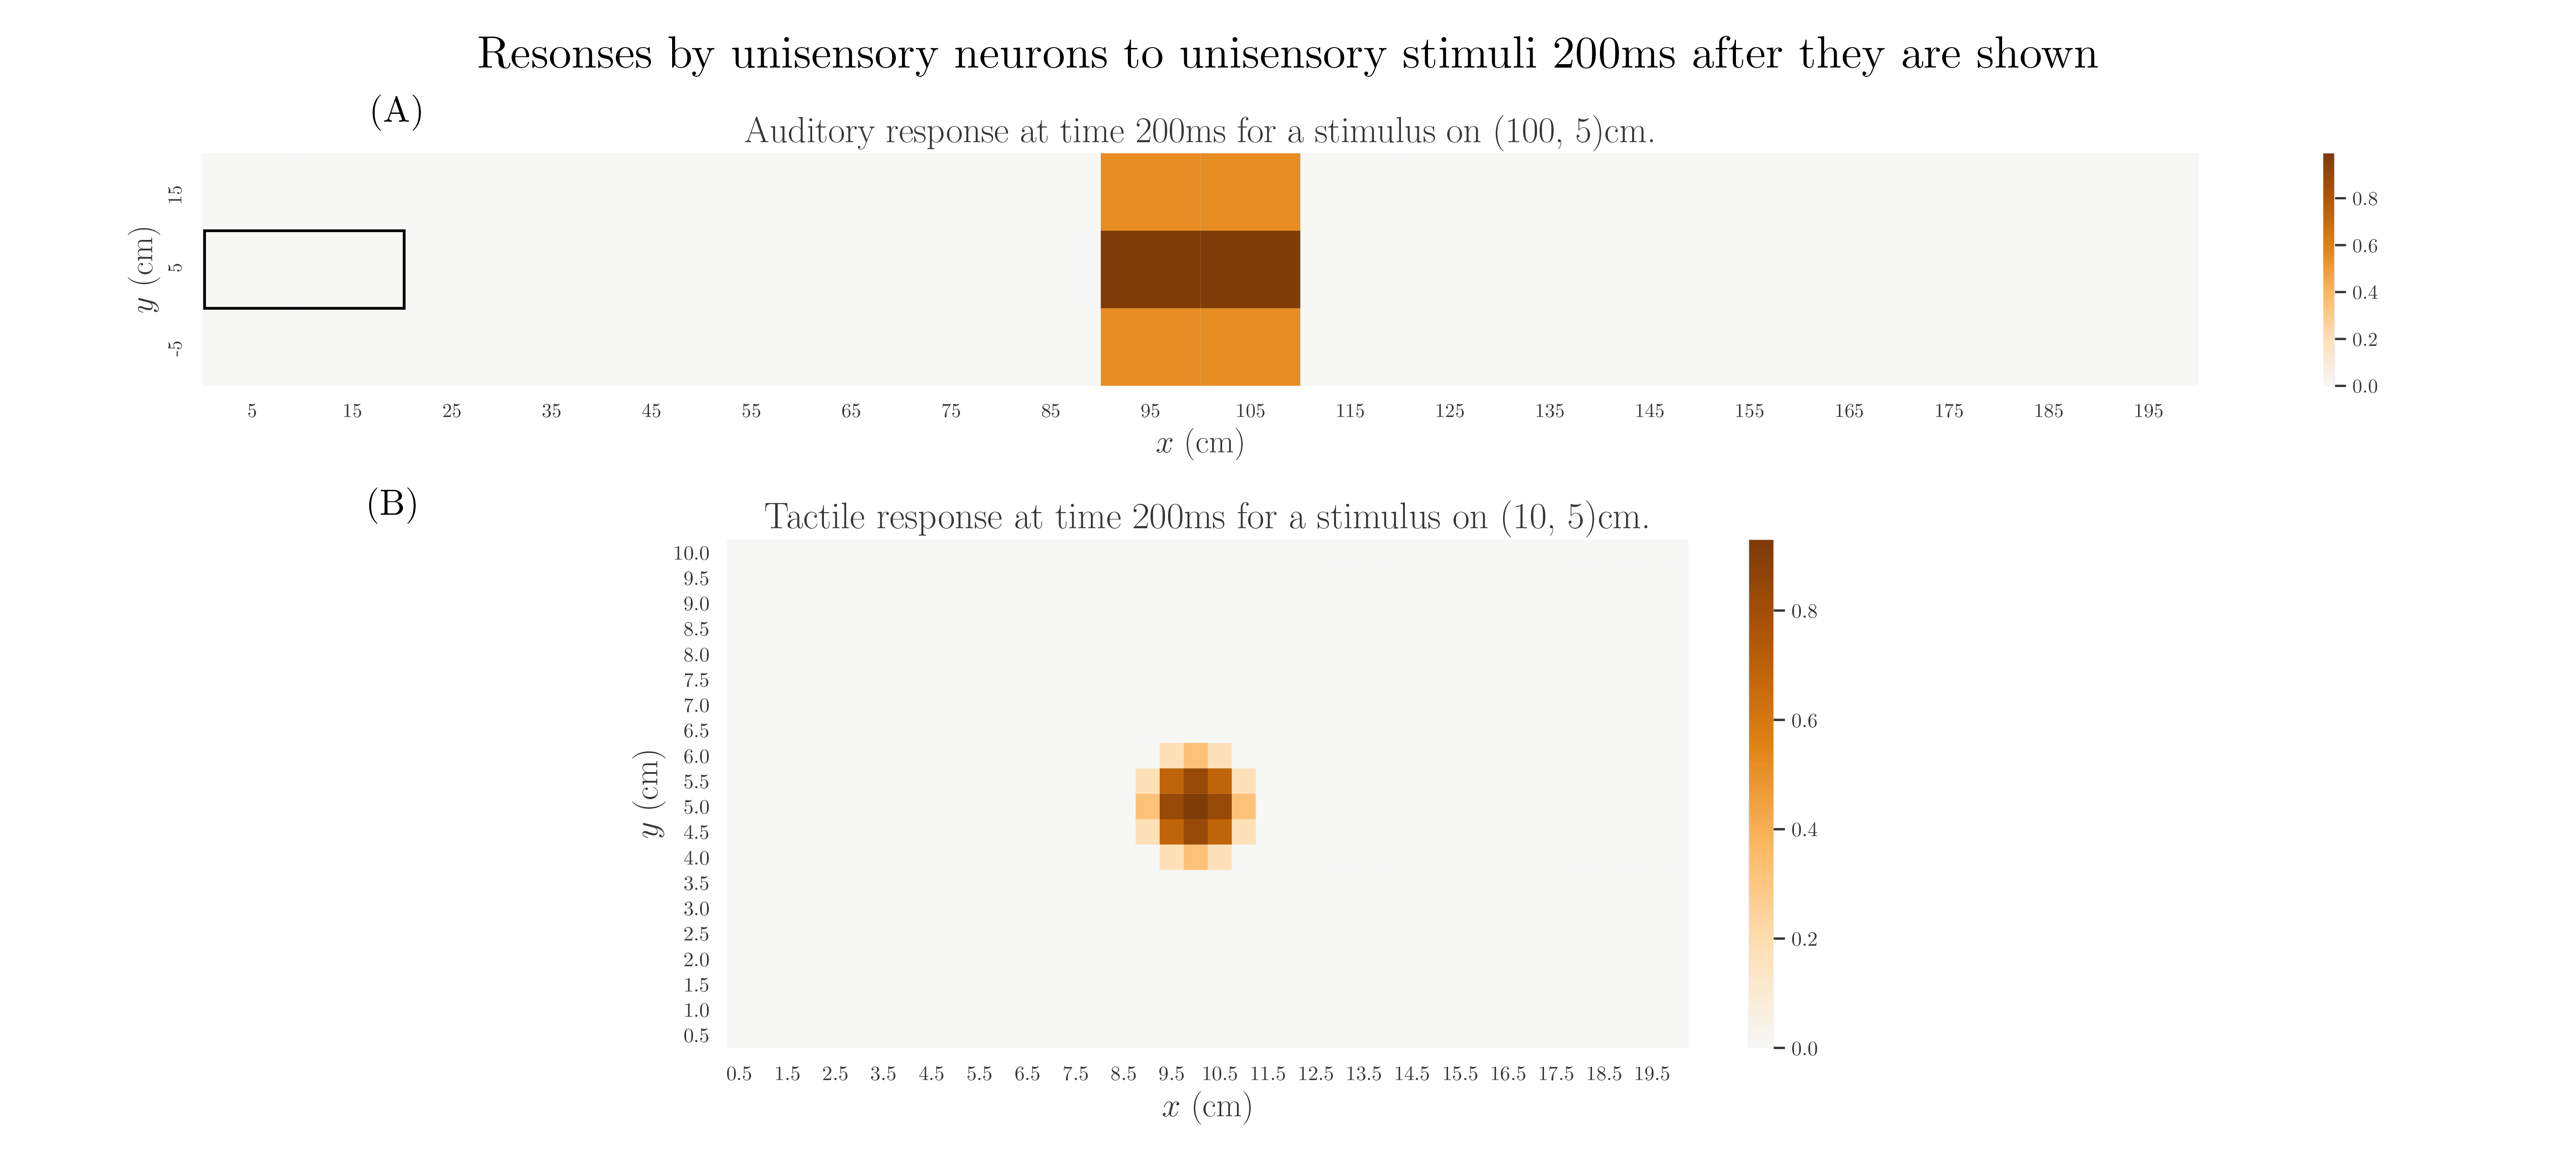
\includegraphics[width=1.2\linewidth]{fig/3-3-1.png}
	\caption{Responses of unisensory areas to unisensory stimuli 200ms after they are shown. Figure \textit{(A}) shows the response of the auditory area for an auditory stimulus placed at coordinates $(100, 5)$cm. Similarly, figure \textit{(B)} shows the response of the tactile area at coordinates $(10,5)$cm.}
	\label{fig:3.3.1}
\end{figure}

\subsection{The role of the feedforward connection}

The role of the feedforward connection was obtained by plotting the responses of the unisensory neurons for different values of $L_{in}^s \mathrm{\, and \,} L_{ex}^s$. These are shown in figure \ref{fig:3.3.3}.

\begin{figure}[h!]
	\centering
	\hspace*{-0.6in}
	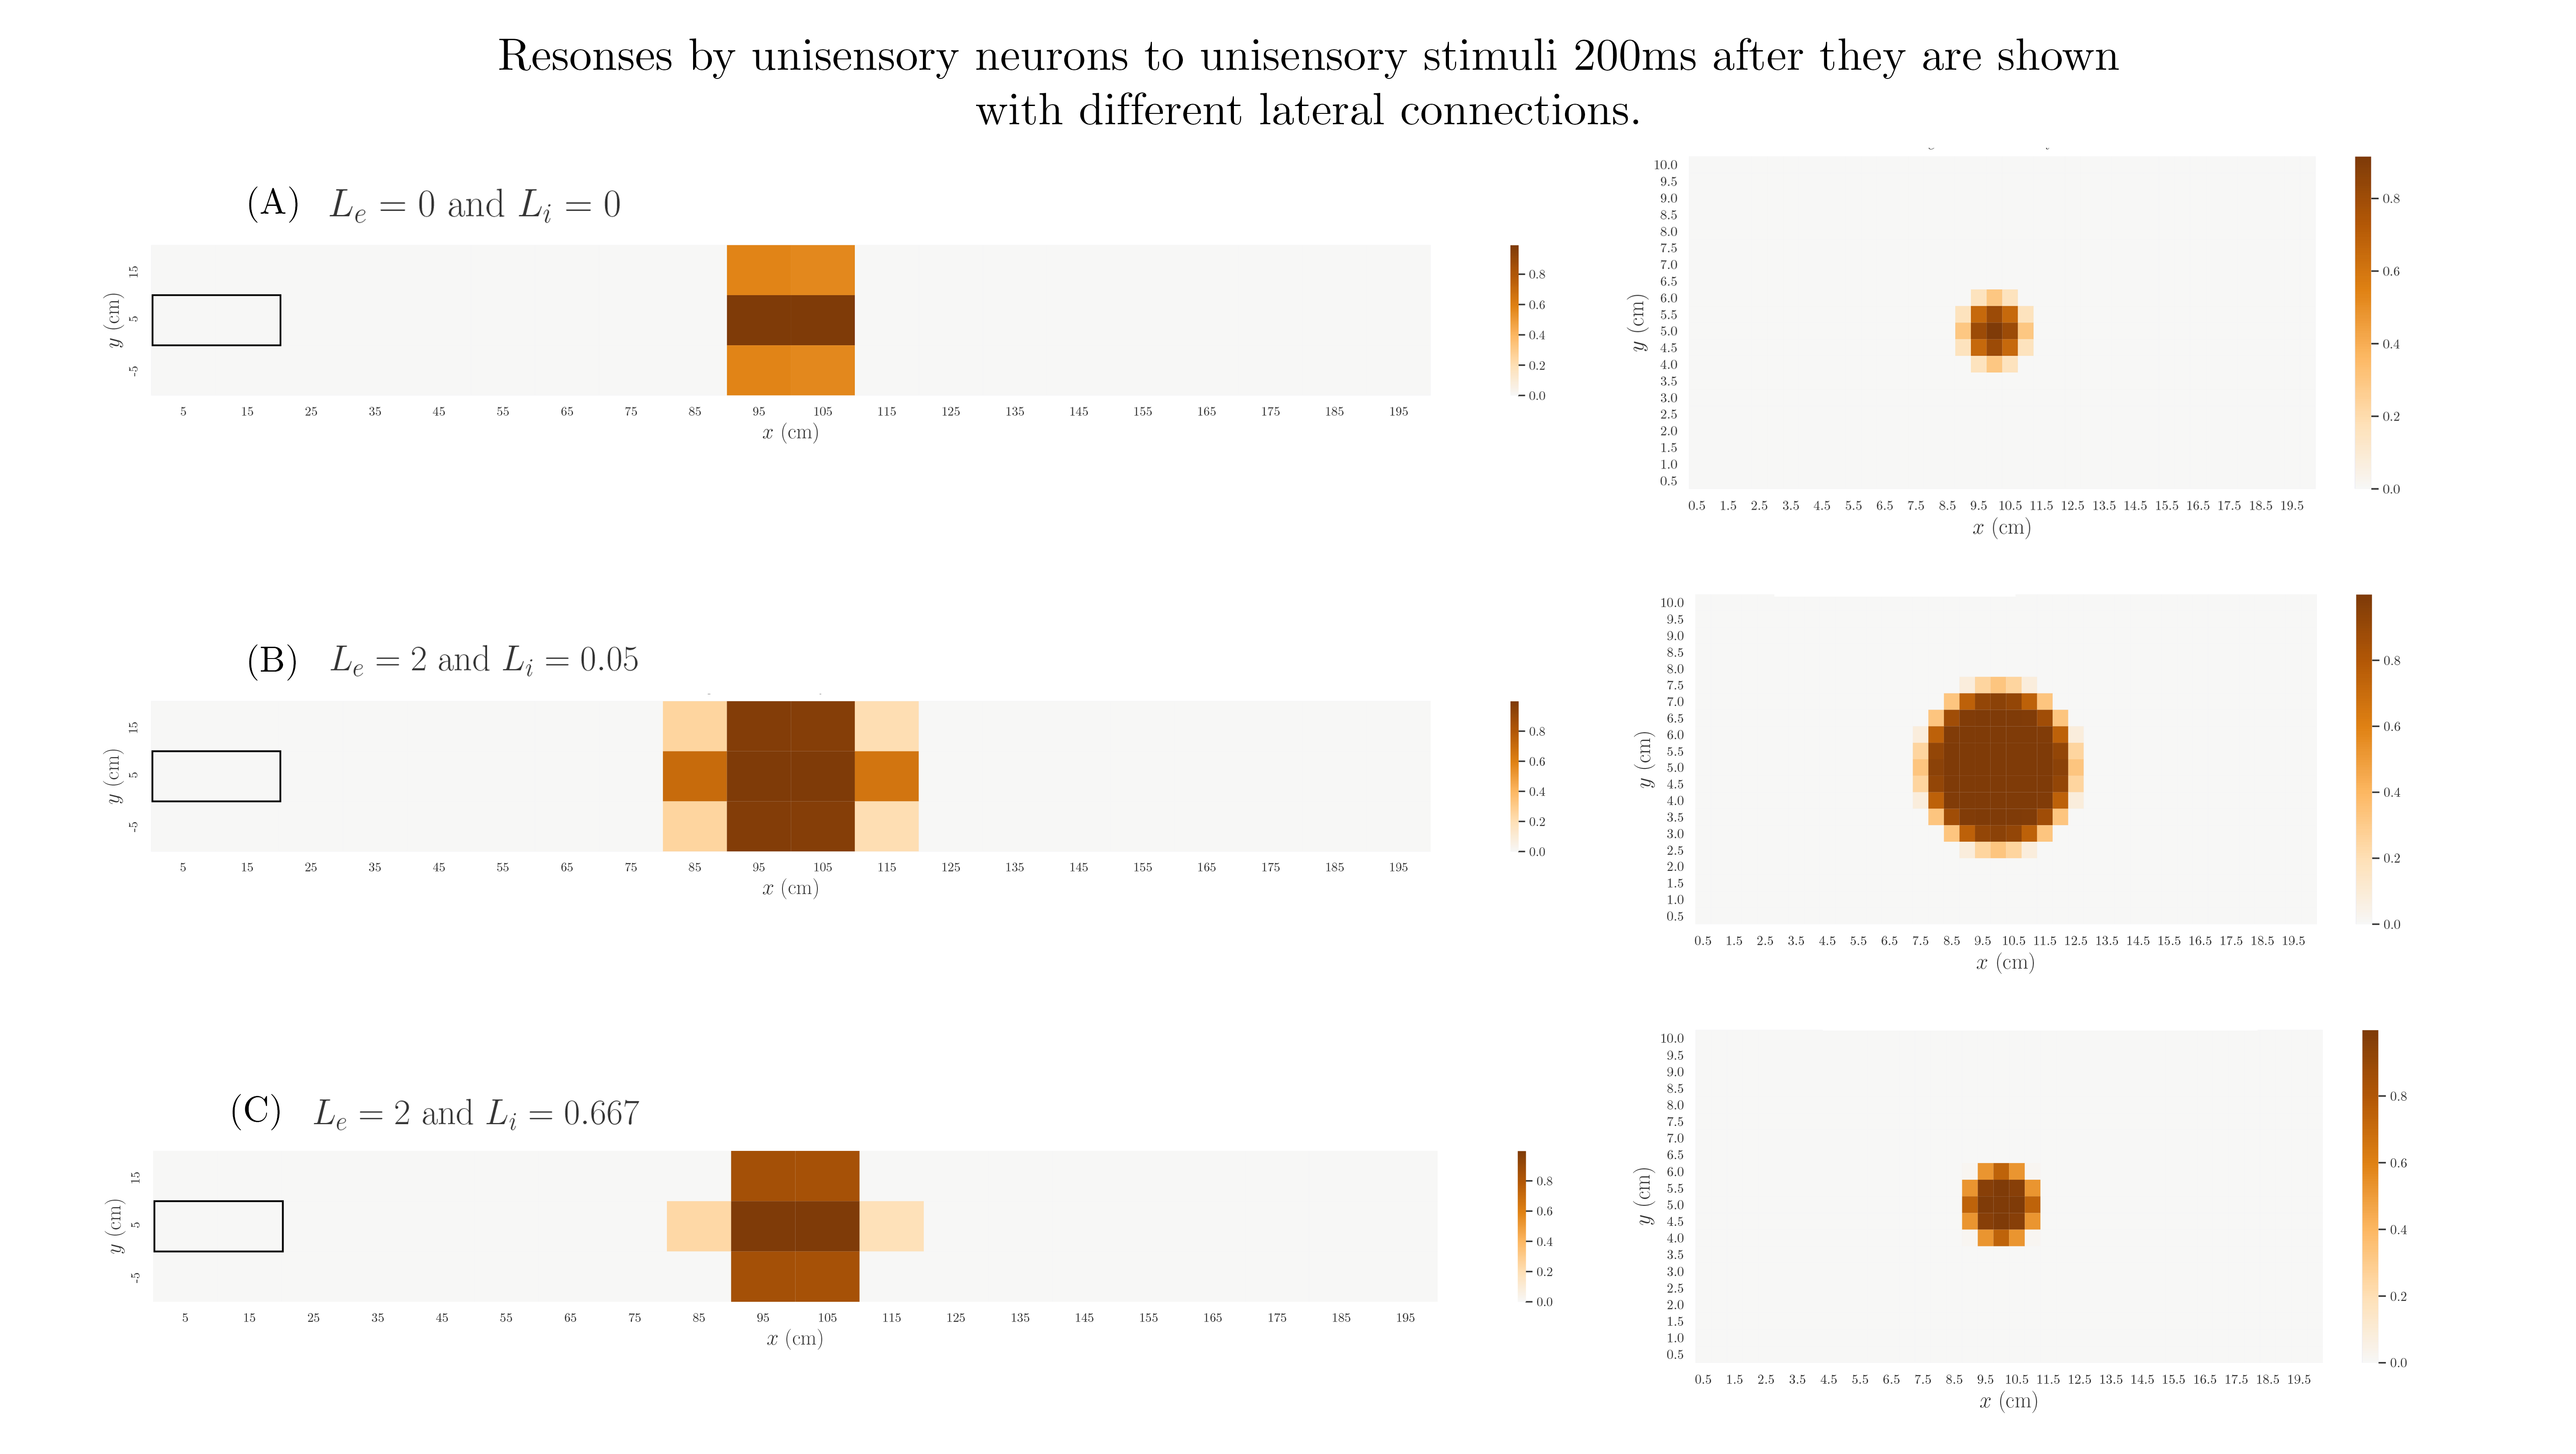
\includegraphics[width=1.15\linewidth]{fig/3-3-3.png}
	\caption{Responses for the unisensory areas for stimulu placed at $t=200$ms and impulses placed on $(10,5)$cm and $(100, 5)$cm respectively for different values of lateral synapses. }
	\label{fig:3.3.3}
\end{figure}

The first trial was eliminating the lateral connections (figure \ref{fig:3.3.3} \textit{(A)}). This resulted in less activity in the neurons surrounding the neuron with receptive field centre closest to the stimulus centre.

Then the excitatory amplitude was augmented, while the inhibitory amplitude stayed the same. Figure \ref{fig:3.3.3} \textit{(B)} shows that for both types of stimuli, the corresponding neurons close to the stimulus centre got more exctied than with the default parameters, and even neurons that did not fire before started firing.

Lastly, both the excitatory and inhibitry amplitudes were excited, but maintaing the ratio $\frac{L_{ex}^s}{L_{in}^s}$. Figure \ref{fig:3.3.3} \textit{(C)} shoes that the pattern is very similar to when using the default parameters. However, in these scenario the surrounding neurons responded less.

The lateral connection, therefore, performed as expected. Increasing the amplitude of the excitatory neurons yielded to more activity in the neurons surrounding the stimulus, and removing the lateral stimuli made the responde more concentrated around the centre.

\subsection{The effect of the auditory stimulus location on the multisensory neuron}

The effect of the position of the auditory stimulus on the activity of the multisensory neuron can be observed in table \ref{tab:1}.

\begin{center}
 \begin{table}
 \begin{tabular}{|c | c | c |}
 \hline
 Stimulus coordinates & time such that $z > 0.1$ (s) & time such that $z > 0.9$ (s) \\ [0.5ex]
 \hline\hline
 (20, 5) & 30.4 & 37.2 \\
 \hline
 (60, 5) & 30.4 & 37.2 \\
 \hline
 (100, 5) & 38.4 & 48.0  \\
 \hline
 (140, 5) & 39.6 & 50.0 \\
 \hline
 (180, 5) & 40.0 & 50.0  \\ [1ex]
 \hline
 \end{tabular}
 \caption{Time taken for the multisensory to reach 10 and 90 \% of its steady-state activity for different $x$ coordinates of the auditory stimulus.}
 \label{tab:1}
 \end{table}
\end{center}

$x$ coordinates 20 and 60 the times taken are the same, as they lie within the limit that makes their corresponding feedforward weights constant. However, as the $x$ coordinate travels further away from the hand, the times taken by the multisensory neuron to reach the desired activity increase. The biggest increase is between 60 and 100, which is consistent with the sigmoid that will be fit in section \ref{sec:4}.

\subsection{Role of the feedback connectivities}

The feedback connectivities go from the multisensory neuron to the neurons in the unisensory areas. The first step in testing their effect was to run the simulation only with a tactile stimulus, and then checking the final auditory dynamic-state, $q_{t=200}^a$, and vice-versa.

Running the simulation with a tactile stimulus on coordinates $(10, 5)$cm resulted in a final auditory dynamic-state of 2.5.

When ran with an auditory stimulus in $(20, 5)$cm, inside the peri-personal space boundary, the resulting tactile dynamic-state was 1.0.

Therefore, the feedback connectivities can cause the unisensory neurons to have some activity (about 10 to 20\% of what they need to fire), even if no stimulus of that type was presented.

The next step was to test the reaction times of the tactile neurons with an auditory stimulus (which would cause them to have more feedback input) and without. Running the simulation without the auditory stimulus had a reaction time of 85.6ms, while doing it with a synchronous auditory stimulus on $(40, 5)$cm had a shorter reaction time of 78.8ms.

Therefore, the feedback connections act like a bridge between both unisensory areas. If triggers some activity in the tactile area when there was been a stimulus in the auditory area, and vice-versa.

\section{Influence on the reaction times}
\label{sec:4}

\subsection{Activity of the multisensory neuron as a function of time}

The activity of the multisensory neuron as a function of time was computed for different $x$ coordinates in the auditory space to see how the distance from the auditory stimulus to the hand influences the activation of the multisensory neuron.

\begin{figure}[h!]
	\centering
	\hspace*{-1.5in}
	
\includegraphics[width=1.5\linewidth]{fig/4-1.png}
	\caption{Activity of the multisensory neuron ($z$) as a function of time for different positions of the auditory stimulus. For all plots, there is a tactile stimulus placed at $(10,5)$cm.}
	\label{fig:3.4.1}
\end{figure}

The results can be seen in figure \ref{fig:3.4.1}. For $x^a=19$, $x^a=35$ and $x^a=55$ the activity is exactly the same. This can be explained because all the $x$ coordinates lie within the limit where the feedforward weight is constant. It can be seen, however, that the activations are slower as the distance increases further.

\subsection{Reaction times and boundaries of the PPS}

The reaction times, $\mathrm{RT}^{90\%}$ are defined as the time at which the tactile neurons reach 90\% of their final activity. These values were obtained by
\begin{enumerate}
  \item Summing over all the activations in the tactile area at $t=200$ms, let $Z_{200}$.
  \item At each time-step, compute the sum of all the activations $Z_i$.
  \item The reaction time will be the first $i$ such that  $Z_i \geq Z_{200} \times 0.9$.
\end{enumerate}

Finally, in order to obtain more realistic values for the reaction times, we used

\[RT = 3\mathrm{RT}^{90\%} + 60, \]

as given in the assignment sheet.

\begin{figure}[h!]
	\centering
	\hspace*{-1.9in}
	
\includegraphics[width=1.5\linewidth]{fig/4-2.png}
	\caption{Reaction times as a function of the $x$ coordinate of the auditory stimulus, with a tactile stimulus placed at the centre of the tactile area.}
	\label{fig:3.4.2}
\end{figure}

Figure \ref{fig:3.4.2} shows the reaction times as a function of the $x$ coordinate of the auditory stimulus, with a tactile stimulus placed at the centre of the tactile are as well.The values of $x^a$ range from 10 to 190cm in steps of 10cm. The upper limit of 190cm was chosen over the 91cm, as stated in the assignment sheet, to show the full sigmoidal shape.The sigmoidal shape is very similar to figure 4 \textit{(B)} in \cite{Serino2015}, but flipped horizontally and with a different scale. Nevertheless, the shape is consistent with Serino's findings, and it suggests that the peri-personal boundary lies at approximately 85cm from the hand.

In order to understand further the boundary of the peri-personal space, a sigmoid was fit to the data (figure \ref{fig:3.4.3}).

\begin{figure}[h!]
	\centering
	\hspace*{-1.9in}
	
\includegraphics[width=1.5\linewidth]{fig/4-3.png}
	\caption{Reaction times as a function of the $x$ coordinate of the auditory stimulus, with a tactile stimulus placed at the centre of the tactile area, and a sigmoid of best-fit.}
	\label{fig:3.4.3}
\end{figure}

Equation \ref{eq:1}, taken from equation 10 in the assignment sheet, the sigmoid to map form the dynamic states $q$ to the rates $z$, was used as a template:

\begin{equation}
  F(x) = \frac{b_{\mathrm{min}} + b_{\mathrm{max}} \times \exp{(x - x_{\mathrm{centre}}) * \mathrm{steepness}}}{1 + \exp{(x - x_{\mathrm{centre}}) * \mathrm{steepness}}}
  \label{eq:1}
\end{equation}

The parameters to fit the data properly were found by trial and error:

\[b_{\mathrm{min}} = 296.0, \;
  b_{\mathrm{max}} = 314.6, \;
  x_{\mathrm{centre}}= 88, \text{ and } \;
  \mathrm{steepness} =  0.11\]

As $x_{\mathrm{centre}}$ and $\mathrm{steepness}$ are defined as the centre of the sigmoid and the steepness at the centre according to the assignment sheet the PPS boundary and the steepness of the boundary are 88cm and 0.11 respectively.

\section{Differences in mental illness}

In schizophrenia it is found that the PPS are narrower and the slope is sharper \cite{dicosmo}. One of the suggested hypotheses is pruning of the weakest feedforward and feedback connectivities. In order to explain how this impairment could affect the PPS boundary, the pruning was implemented in the model. 

All the neurons in the tactile area have the same connectivity weights to the multisensory neuron, therefore those were not pruned. For pruning in the auditory weights, the 60\% smallest weights were set to 0, which represents the impairment of these weakest connections. 

\begin{figure}[h!]
	\centering
	\hspace*{-1.9in}
	
\includegraphics[width=1.5\linewidth]{fig/3-5.png}
	\caption{Reaction times as a function of the $x$ coordinate of the auditory stimulus, with a tactile stimulus placed at the centre of the tactile area, and a sigmoid of best-fit. The auditory feedback and feedforward weights have a pruning of the 60\% weakest connections.}
	\label{fig:3.5}
\end{figure}

Figure \ref{fig:3.4.3} was replicated using the pruned auditory feedforward and feedback connectivity weights. The sigmoid was fit using the same technique, and the parameters were again found by trial-and-error. The results can be seen in figure \ref{fig:3.5}. 

The parameters for the best-fit sigmoid with pruning are

\[b_{\mathrm{min}} = 296.2, \;
  b_{\mathrm{max}} = 317, \;
  x_{\mathrm{centre}}= 78, \text{ and } \;
  \mathrm{steepness} =  0.3\]

The boundary of the PPS is therefore 10cm narrower, and the steepness is almost 3 times greater. 

Individuals with schizophrenia frequently report experiencing bodily self-disturbances such as sudden changes in size and shape of the body and flexible or porous body boundary \cite{VR}. This phenomenon could be explained with the disturbance in the PPS due to impairments in the unisensory-multisensory connectivities. 

In further experiments it would be insightful to extend the pruning model further to random impairments, not just the weakest connections, including in the tactile area. It would also be worth considering and combining other hypotheses to explain the reduction of the PPS, such as impairments in the lateral unisensory connectivities. 

\bibliography{bib}

\end{document}
